
%%%%%%%%%%%%%%%%%%%% file icsc2024_template.tex %%%%%%%%%%%%%%%%%%%%%
% based on icsc2017 / 2022 template updated by Alex Hofmann for icsc2024 -- Nov. 2023
%
% This is the LaTeX source for the instructions to authors using
% the LaTeX document class 'llncs.cls' for contributions to
% the Lecture Notes in Computer Sciences series.
% http://www.springer.com/lncs       Springer Heidelberg 2006/05/04
%
% It may be used as a template for your own input - copy it
% to a new file with a new name and use it as the basis
% for your article.
%
% NB: the document class 'llncs' has its own and detailed documentation, see
% ftp://ftp.springer.de/data/pubftp/pub/tex/latex/llncs/latex2e/llncsdoc.pdf
%
%%%%%%%%%%%%%%%%%%%%%%%%%%%%%%%%%%%%%%%%%%%%%%%%%%%%%%%%%%%%%%%%%%%


\documentclass[runningheads,a4paper]{llncs}

\usepackage{amssymb}
\setcounter{tocdepth}{3}
\usepackage{graphicx}
% \usepackage{url}
\usepackage{hyperref}
\usepackage[margin=1.1in]{geometry}
\hypersetup{hidelinks}
\newcommand{\keywords}[1]{\par\addvspace\baselineskip
\noindent\keywordname\enspace\ignorespaces#1}

\pagestyle{headings}

\begin{document}

\mainmatter  % start of an individual contribution

% first the title is needed
\title{cloud-5:\\An System for Generating and Publishing Cloud Music}

% a short form should be given in case it is too long for the running head
\titlerunning{Running Title}


% TO GARANTEE THE DOUBLE BLIND REVIEW PROCESS, PLEASE
% KEEP THESE GENERIC AUTHOR NAMES AND INSTITUTIONS

\author{AuthorA\inst{1}\and AuthorB\inst{2} \thanks{I thank Dan Derks for introducing me to Tidal Cycles and Felix Roos for answering Strudel questions.}}
%
% if the names of the authors are too long for the running head, please use the format: AuthorA et al.
\authorrunning{AuthorA and AuthorB (or AuthorA et al. if too long)}

% the affiliations are given next; don't give your e-mail address
% unless you accept that it will be published
\institute{InstituteA \and InstituteB\\ \email{your.email@yourdomain.com}}

%
% NB: a more complex sample for affiliations and the mapping to the
% corresponding authors can be found in the file "llncs.dem"
% (search for the string "\mainmatter" where a contribution starts).
% "llncs.dem" accompanies the document class "llncs.cls".
%


\maketitle

% Should be 150 to 350 words.
\begin{abstract}
The advent of the World Wide Web, the standardization of HTML with adequate support for computer graphics and audio, and the introduction 
of WebAssembly as a low-level language and browser-hosted runtime for any number of computer language compilers, have combined to create an environment well suited to the \emph{online} production, publication, and presentation of art music, visual music, and 
related media at a \emph{professional} standard of technical quality. A piece of music on the World Wide Web no longer need be merely 
a link to a downloadable soundfile or video, or even to an audio or visual stream. A piece can, indeed, be its own ``app" that is live code running at near native speed  in the listener's Web browser. I call this kind of music \emph{cloud music} because it exists only in the ``cloud,'' the omnipresent computing infrastructure of the Web. I argue that this creates an entirely new environment for music that may, in the future, develop its own social context and function as an alternative means of disseminating art music in addition to live performances, discs, streams, and downloads. Here, I present and demonstrate \emph{cloud-5}, a collection of Web components for producing cloud music including, among other things, fixed medium music, music that plays indefinitely, visuals that generate music, music that generates visuals, interactive music, and live coding. cloud-5 includes a WebAssembly build of the sound programming language and software synthesis system Csound, a WebAssembly build of the CsoundAC library for algorithmic composition including chords, scales, and voice-leading, the live coding system Strudel, and supporting code for menus, event handlers, GLSL shaders, and more. A cloud-5 piece thus exists as an HTML page that embeds Csound code and/or score generation code and/or Strudel code and/or GLSL code, in the context of a static Web site that can be served either locally (for composing and performing) or remotely on the World Wide Web (for publication).
\keywords{html5, webassembly, csound, algorithmic composition, visual music, live coding}
\end{abstract}

\section{Introduction}

The World Wide Web was invented for the purpose of publishing scientific information by any scientist, to any scientist. It was then co-opted by American business interests for the purpose of selling to consumers. Along the way, it became a conduit for the wholesale theft of intellectual property in the form of illegal downloads of recorded music, films, and computer games. Then it became the major platform for social media, another (disguised) form of selling to consumers while taking their personal data. Indeed, most people's use of the Web has been increasingly funneled through Google search and various social media platforms, which are highly proprietary and far from open. Yet, at every step along this tortuous path, the original inventions that created the World Wide Web, including packet-switched networking (especially TCP/IP) and the Web browser itself, based on  Web standards (including HTTP, URLs, HTML, MIME types, JavaScript, and now WebAssembly), have remained non-proprietary, decentralized, backwards compatible, and more or less open. In fact, driven by both entrepreneurship and the competitive pressure to show ever more appealing ads, the power of Web browsers has increased to the point of providing the equivalent of a game engine and an operating system, running only about 1.5 to 2.5  times as slowly as native C code.

I would go so far as to say that the establishment of Web standards is one of the most fortunate things that has ever happened, because it preserves essential freedoms in face of a rather remarkable level of skilled greed (I remain wary, however, that private interests will end up hijacking these standards and manipulating them to be less open).

Now to music. Music now has, in spite of everything, thanks to Web standards and the growing capabilities of browsers, a new platform that provides both novel power to composers and novel availability to audiences. This is what I call \emph{cloud music}: computer music that runs in Web browsers. Not downloads, not streams, but autonomous programs that synthesize music and visuals in real time with the option of interacting with the audience, performing endlessly, producing endless variations, and communicating across the world. Such music can be free, or secured for paid subscriptions, or supported by advertising. 

The audio resolution in cloud-5 is the same as that of WebAudio: 48,000 frames per second of floating-point samples in 128 frame buffers. Although studio software can offer even higher resolution, WebAudio does operate within the recognized range of professional audio production quality. Furthermore, Csound can interpolate samples within the 128 frame buffers.

For examples of cloud music, one may look to online computer games with procedural audio, the Strudel live coding system, or my own compositions produced using the subject of this paper, cloud-5.

\section{Use Cases and Examples}

\begin{description}
\item[Composition] The cloud-5 system is useful for the composition of electroacoustic music because it contains very powerful facilities. These include all the astonishing capabilities already built into every standard Web browser, a complete WebAssembly build of Csound, a complete WebAssembly build of the CsoundAC algorithmic composition library, the complete Strudel live coding system which can render audio using either Csound or its own built-in sampler and synthesizer, and any other module that will run in a Web browser. All of these facilities are completely cross-platform. That makes cloud-5 far and away the easiest computer music system of comparable power to install and configure: unzip it somewhere and run a local Web server in that directory. 
\item[Fixed Pieces] These are similar to fixed medium pieces of electroacoustic music. When the user starts the piece, it plays audio until the score ends. 
\item[Always-On Pieces] Similar to fixed pieces; but once started, always-on pieces play indefinitely. By using randomization or fractals, always-on pieces can play indefinitely without any repetition.
\item[Interactive Pieces] Similar to fixed pieces or always-on pieces; but once the piece is started, the user interface provides controls with which the user may steer some aspects of the composition or rendering.
\item[Live Coding] Similar to interactive pieces; but the user has \emph{complete} control over the composition in the Strudel REPL, and can create entirely new compositions or engage in lengthy improvisations.
\item[Music Visualization] Similar to the other pieces above, but a GLSL shader displays a visualization controlled by the audio on the background of the piece, and this visualization can be made full screen.
\item[Visual Music] Similar to music visualization, but the video buffer is periodically downsampled or otherwise processed to produce fragments of Csound score, which are rendered by Csound in real time.
\item[Network Pieces] Any of these types of pieces can request additional resources from the Internet, or be controlled remotely.
\end{description}

\section{Basic Design}

The cloud-5 user interface consists of a main menu running across the top of the page. Clicking on a button can start or stop performance, or show/hide various overlays that fill the rest of the page. 

The cloud5-system is constructed as a library of Web components in the form of HTML custom elements, which encapsulate code and even some styling within each HTML element. This makes it much easier for users not familiar with the details of HTML or JavaScript to write cloud-5 pieces. The user includes these custom elements in the HTML code like any other elements, adds user-defined code such as a Csound orchestra or Strudel patch, and hooks the parts up together using a little JavaScript. Code folding regions make it easier to organize the code and to see only the part that is being edited. To make it easier for users to construct pieces, a naming convention is used. Names ending in \texttt{\_overlay} denote Web. components, and names ending in \texttt{\_addon} denote things that the user must or map provide, including code (JavaScript, Csound, Strudel, GLSL), parameters, and others.

\subsection{Components}

Currently, cloud-5 consists of the following custom elements and user addons:

\begin{description}
\item[\texttt{<cloud5-piece>}] This custom element defines the main menu of the piece and its event handlers, instantiates Csound and/or Strudel as required, starts and stops performances, hosts a controls submenu, and defines some helper JavaScript code.
\item[\texttt{<cloud5-piece>.csound\_code\_addon}]  This is user-defined code as a multi-line JavaScript string containing the complete text of a Csound .csd file (which can be quite large).
\item[\texttt{<cloud5-piece>.control\_parameters\_addon}]  This a user-defined JavaScript object whose fields have the names and initial values of Csound control channels.
\item[\texttt{<cloud5-piece>.menu\_folder\_addon}]  The user calls this with the name of a new folder to be added to the controls menu of the piece.
\item[\texttt{<cloud5-piece>.menu\_slider\_addon}]  The user calls this with the name of a new slider control to be added to the controls menu, along with its Csound channel name, lowest value, highest value, and the folder to which the slider will be added.
\item[\texttt{<cloud5-piece>.score\_generator\_function\_addon}]  This is user-defined code in the form of a JavaScript function that will be called at the start of performance to generate a CsoudAC score to be performed by Csound. 
\item[\texttt{<cloud5-piano-roll>}] This custom element is an overlay that draws a three-dimensional piano roll display of a generated CsoundAC Score. During performance, the piano roll shows the current position in the Score with a moving ball. It is possible to zoom in and out of the piano roll, drag it around, rotate it, and so on.
\item[\texttt{<cloud5-strudel>}] This custom element is a popup IFrame that shows the Strudel REPL, in which the user can do live coding of the Strudel patch during performance. The Strudel REPL has its own real-time piano roll display, and highlights the currently active functions in the Strudel code.
\item[\texttt{<cloud5-strudel>.strudel\_code\_addon}] This is user-defined code as a multi-line JavaScript string containing a complete Strudel patch to be performed by the piece.
\item[\texttt{<cloud5-shadertoy>}] This  custom element is an overlay that shows a canvas displaying a GLSL shader. This shader can be used to visualize audio, to produce notes for Csound to perform, and so on. The element is designed to support the easy adaptation of shaders developed in the ShaderToy Web site.
\item[\texttt{<cloud5-shadertoy>.shader\_parameters\_addon}] This is a user-defined Javascript object with the following fields:
\begin{description}
\item[\texttt{fragment\_shader\_code\_addon}] Contains user-defined GLSL code to be compiled for display on the canvas of the shader overlay.
\item[\texttt{vertex\_shader\_code\_addon}] May contain user-defined GLSL code to be compiled for display on the canvas of the shader overlay; there is a default value that includes the entire canvas.
\item[\texttt{set\_uniforms\_function\_addon}] This may be set to user-defined code in the form of a JavaScript function that will be called before every shader animation frame to set uniforms that can be used to control the shader; commonly used to implement an audio visualizer.
\item[\texttt{get\_attributes\_function\_addon}] This may be set to user-defined code in the form of a JavaScript function that will be called after every shader animation frame to read attributes that can be used by the piece; for example, to sample the visuals and translate them to Csound notes to be played.
\end{description}
\item[\texttt{<cloud5-log>}] This custom element is an overlay that presents a scrolling list of runtime messages from Csound and/or other sources.
\item[\texttt{<cloud5-about>}] This custom element is an overlay that presents license information, authorship, credits, program notes, and so on.
\end{description}

\section{An Example Piece}

The following example is a simple piece that nevertheless uses many of the custom elements presented above. The code is folded to show only the high-level elements and how they are connected together.

\subsection{Score Generator}
\subsection{Csound Orchestra}
\subsection{Strudel Patch}
\subsection{Controls}
\subsection{Audio Visualizer}
\subsection{About}

\section{Best Practices}

The cloud-5 system is designed for making permanent works of music -- pieces that will always play, even in the far future (assuming that the Web standards continue to be versionless and backwards-compatible, as they have been for 35 years). In other words, cloud-5 is not at all a general purpose Web development system, and therefore pieces should not be developed in the standard way.

\begin{itemize}
\item Use only local, static resources (e.g., do not use content distribution networks, but rather download all required scripts, etc., to the Web directory). This ensures pieces will continue to function indefinitely, and will not break due to library API changes or missing links.
\item Use no tooling (e.g. no rollups); edit pieces directly in the Web directory. This ensures that pieces will not break due to tooling changes, and will be easy to debug.
\item As far as possible, keep all components and resources of a piece in one HTML file, e.g. embed Csound orchestras and Strudel patches in the HTML code.
\end{itemize}

This is a \LaTeX{} template to be used, together with the included Springer
class file \texttt{llncs.cls}, for the preparation of manuscripts for the
\textit{7\textsuperscript{th} International Csound Conference
\textemdash{} ICSC2024}.

The maximum paper length is four pages including abstract, figures, tables
and eventual references. An additional fifth page is accepted provided it
\textit{only} includes references.

To guarantee the double blind review process, manuscripts should not include
the author names nor affiliations. Please keep the generic names included in the
template.

\section{Paper Preparation}

When using \LaTeX\ together with the provided document class file, the text
is typeset automatically in Computer Modern Roman (CM) fonts. Please do
\emph{not} change the preset fonts or their size, or modify the class file
in any way.

Italic type may be used to emphasize words in running text. Bold type and
underlining should be avoided.

We recommend using the commands \verb+\label+ and \verb+\ref+ for
cross-references, the commands \verb+\bibitem+ and \verb+\cite+ for
references to the bibliography, and the command \verb+\url+ for URL
hyperlinks.


\subsection{Headings}

Only two levels of structure should be used throughout the document,
corresponding to the \verb+\section+ and \verb+\subsection+ sectioning
commands.

Headings should be capitalized, i.e., nouns, verbs, and all other words
except articles, prepositions, and conjunctions should be set with an
initial capital. Words joined by a hyphen are subject to a special rule: if
the first word can stand alone, the second word should be capitalized.

Here are some examples of headings: ``Developing a User-Friendly
Interface'', ``Processing Multi-track Audio Files with Granular Techniques''.

\subsection{Figures}

For integrating figures into the source file we recommend using the
standard \LaTeX{} \verb+graphics+ or \verb+graphicx+ package. These provide
the \verb+\includegraphics+ command. Please center the figures by using the
\verb+\centering+ declaration. Fig.~\ref{fig:example_1} shows an example.

\begin{figure}
\centering
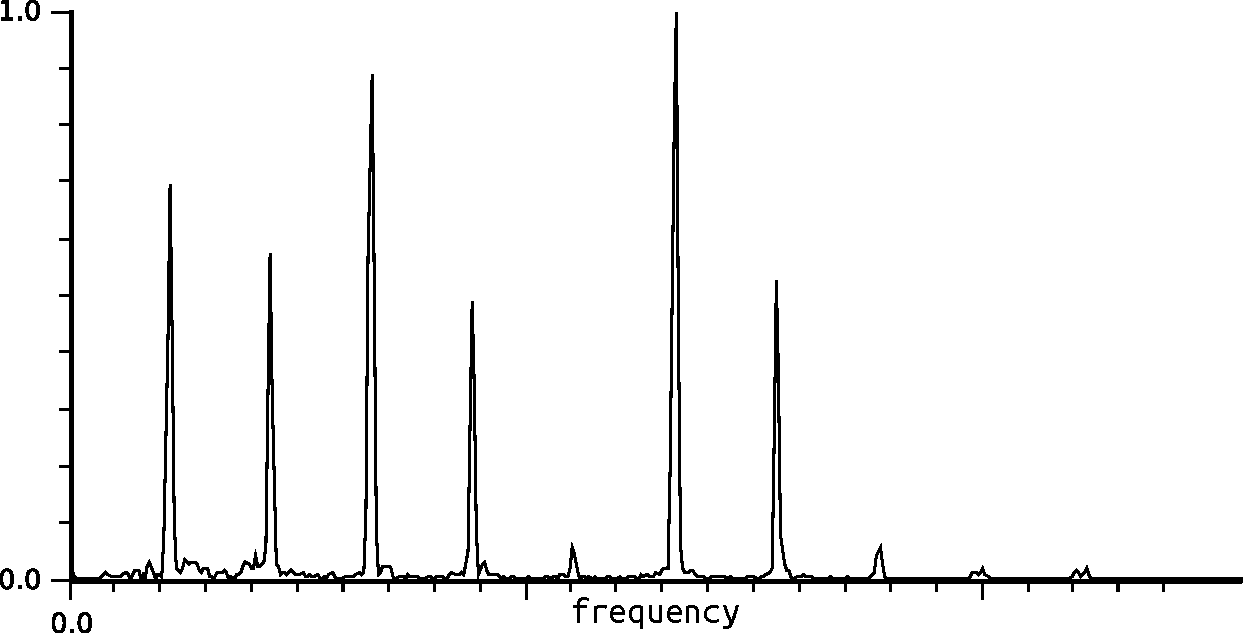
\includegraphics[width=0.90\linewidth]{test_image-1.pdf}
\caption{Spectrogram of a piano note A3 in vector graphics (PDF).}
\label{fig:example_1}
\end{figure}

For line drawings, vector graphics file formats like EPS or PDF are preferred
when available. When including figures in raster graphics file formats like
JPG or PNG, please try to generate an image of the appropriate size and
quality. (See Fig.~\ref{fig:example_2})

Figures should be numbered and should have a caption which should always be
positioned \emph{under} the figures, in contrast to the caption belonging
to a table, which should always appear \emph{above} the table; this is
simply achieved as matter of sequence in your source.

\begin{figure}
\centering
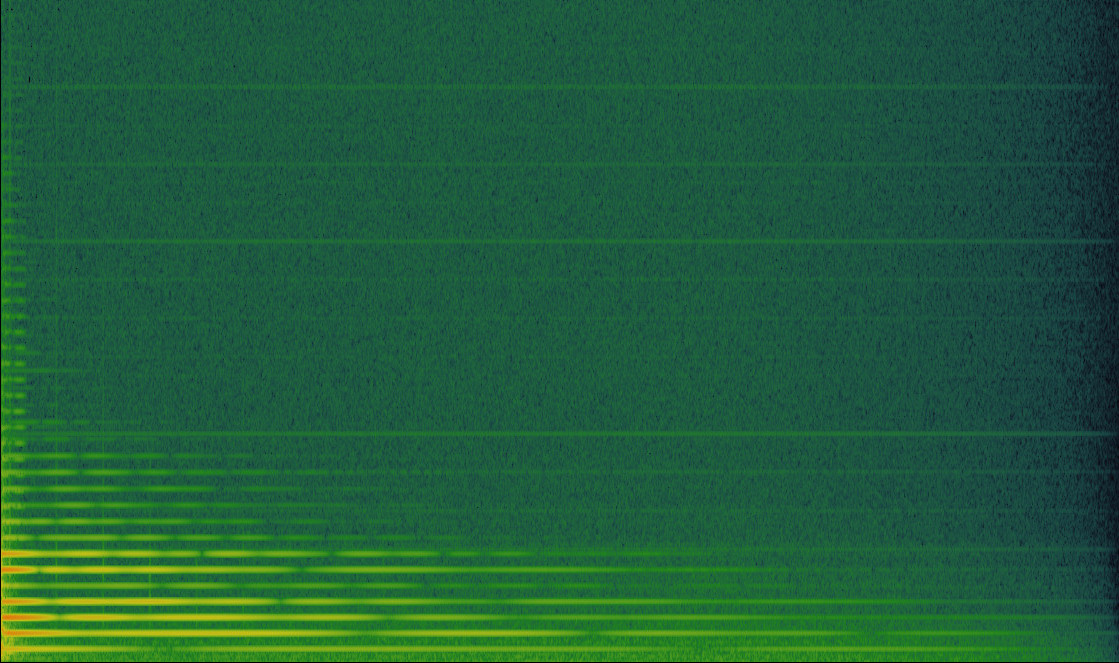
\includegraphics[width=0.90\linewidth]{test_image-2.pdf}
\caption{Spectrogram of the same sound file in raster image (JPG,
1119 x  663 pixels).}
\label{fig:example_2}
\end{figure}

Please define figures (and tables) as floating objects, and avoid using
optional location parameters like ``\verb+[h]+" for ``here".

\paragraph{Remark.}

The proceedings will be distributed only in electronic format, and colored
images are welcome. It would be convenient, however, to make sure that all
the images remain clear and legible when printed in black and white.

\subsection{Footnotes}

The superscript numeral used to refer to a footnote appears in the text
either directly after the word to be discussed or -- in relation to a
phrase or a sentence -- following the punctuation sign (comma, semicolon,
or period).\footnote{Example of a footnote.}

\subsection{Program Code}

Program listings or program commands in the text should use the \verb+verbatim+
environment: \\ \verb+csound -o dac foo.csd+.

\medskip

\noindent
{\it Example of Program Code}
	\begin{verbatim}
<CsoundSynthesizer>
<CsInstruments>

sr     =   48000
ksmps  =   8
0dbfs  =   1

instr  1

idur   =   p3
iamp   =   ampdbfs(p4)
ifreq  =   cpspch(p5)
kamp   linen  iamp, 0.1, idur, 0.3
a1     poscil kamp, ifreq
       out    a1

endin

</CsInstruments>
<CsScore>

i1 0   1   -3   8.00
i1 +   .   -6   8.01
i1 +   .   -4.5 8.07

</CsScore>
</CsoundSynthesizer>
	\end{verbatim}
%
\noindent
{\small Example Csound CSD file.}

\subsection{Citations}

For citations in the text please use square brackets and consecutive
numbers: \cite{jour}, \cite{proceeding} -- provided automatically
by \LaTeX 's \verb|\cite| \dots\verb|\bibitem| mechanism.

\subsection{Page Numbering and Running Heads}

Pages are numbered automatically. If the paper title is too long to serve
as a running head, it will be shortened. A shorter version of the title can
be provided with the \verb+\titlerunning+ command at the beginning of the
\verb+\document+ section.


\section{The References Section}\label{references}

Only references written using the Latin alphabet are accepted. If the title of
the reference uses a different alphabet, please use the transcript or
translation of the title, followed by the original language in parenthesis, e.
g. (in Russian) or (in Chinese).

The following section shows a sample reference list with entries for
journal articles \cite{jour}, books \cite{book1}, \cite{book2}, book chapter
\cite{chapter}, proceedings without editors \cite{proceeding}, as well as a
URL \cite{url}.

\begin{thebibliography}{4}

\bibitem{jour} Lorrain, D.: A panoply of stochastic `cannons'. Computer Music Journal 4(1), 53--81 (1980)

\bibitem{book1} Dodge, C., Jerse, C.: Computer Music: Synthesis, Composition and 
Performance, 2nd edn. Schirmer, New York (1997)

\bibitem{book2} Lazzarini, V. et al.: Csound: A Sound and Music Computing System.
Springer (2016)

\bibitem{chapter} ffitch, J.: Introduction to program design. In: R. Boulanger,
V. Lazzarini (eds.) The Audio Programming Book, pp. 383--430.
MIT Press, Cambridge (2010)

\bibitem{proceeding} Vercoe, B.: Real-Time Csound, Software Synthesis with
Sensing and Control. In: Proceedings of the International Computer Music
Conference, pp. 209--211. Glasgow (1990)

\bibitem{url} Csound Github site, \url{http://csound.github.io}


\end{thebibliography}



\end{document}
